\section{Auswertung}
\label{sec:auswertung}

Zunächst wurde der \hyperref[fig:acrylblock]{Acrylblock} mit einer Schieblehre vermessen,
um später Kontrollwerte zu haben.
Breite und Höhe lauten
\begin{align*}
  b &= \SI{150}{mm} \\
  h &= \SI{80}{mm} \ .
\end{align*}

Der Abstand von der \textbf{c}-Seite wird vor allem bestimmt,
um den Block später besser visualisieren zu können.
Die Tiefe beträgt $\SI{40}{\milli\meter}$,
wird aber für die folgenden Rechnungen ebenfalls nicht benötigt.

Die Messwerte finden sich in \autoref{tab:mess_schieblehre}.

\begin{table}
  \centering
  \caption{Mit der Schieblehre aufgenommene Abstandsmessungen.}
  \label{tab:mess_schieblehre}
  \begin{tabular}{S S[table-format=2.1] S[table-format=2.1] S[table-format=3.1]}
  \toprule
  {Nr.} &
  {von \textbf{a}-Seite} &
  {von \textbf{b}-Seite} &
  {von \textbf{c}-Seite} \\
  \midrule
  \expandableinput{build/tab/mess_schieblehre.tex}
  \bottomrule
  \end{tabular}
\end{table}

In \autoref{tab:mess_ultraschall} sind die mit der Ultraschallsonde aufgenommenen Messwerte angegeben,
welche in den folgenden Abschnitten ausgewertet werden.
Die zwei fehlenden Einträge kommen dadurch zustande,
dass \textbf{4} von \textbf{3} von \textbf{b} aus betrachtet vollständig verdeckt wird.

\begin{table}
  \centering
  \caption{Mit der Ultraschallsonde aufgenommene Messwerte.}
  \label{tab:mess_ultraschall}
  \begin{tabular}{S | S S | S S}
  \toprule
  &
  \multicolumn{2}{c}{Laufzeit $\symup{\Delta}t$ [$\si{\micro\second}$]} &
  \multicolumn{2}{c}{Amplitude $U_A$ [$\si{\volt}$]} \\
  {Nr.} &
  {von \textbf{a}-Seite} &
  {von \textbf{b}-Seite} &
  {von \textbf{a}-Seite} &
  {von \textbf{b}-Seite} \\
  \midrule
  \expandableinput{build/tab/mess_ultraschall.tex}
  \bottomrule
  \end{tabular}
\end{table}

\FloatBarrier
\subsection{Bestimmung der Schallgeschwindigkeit in Acryl}
\label{sec:auswertung:schallgeschwindigkeit}

Die Geschwindigkeit $c$ einer Schallwelle in Acryl kann mit den vorliegenden Messinstrumenten
leicht aus dem in \autoref{eqn:position_fehlstelle} beschriebenen
Zusammenhang von Weg $d$ und Zeit $\symup{\Delta}t$ bestimmt werden.

Aus den in \autoref{tab:mess_schieblehre} und \autoref{tab:mess_ultraschall} aufgelisteten Werten für Abstand und Zeit
wird die Schallgeschwindigkeit in Acryl mittels linearer Regression somit zu $\SI{2763.38(1046)}{\meter\per\second}$ bestimmt. Messwerte und Regressiongerade sind in \autoref{fig:plt:schallgeschwindigkeit} dargestellt.

\begin{figure}[H]
  \centering
  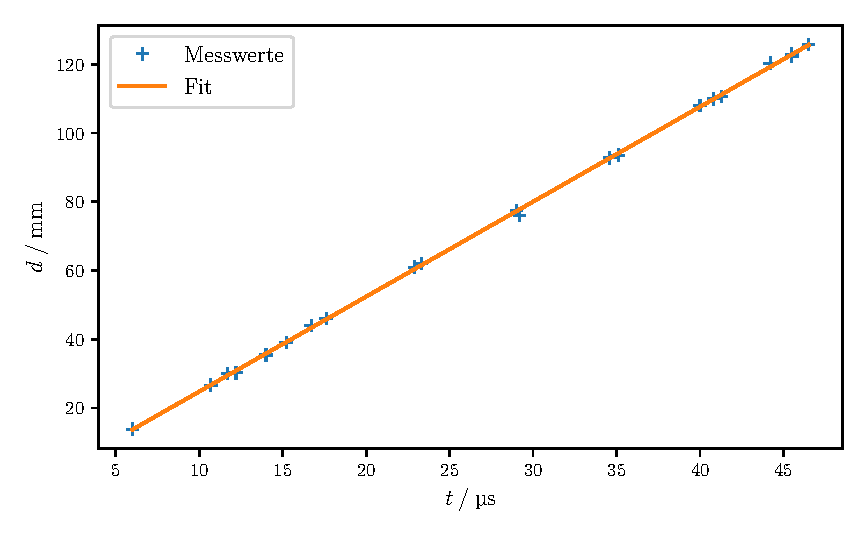
\includegraphics[width=\textwidth]{build/plt/schallgeschwindigkeit.pdf}
  \caption{Zurückgelegte Strecke, aufgetragen gegen die Zeit zum Echo.}
  \label{fig:plt:schallgeschwindigkeit}
\end{figure}

Zur besseren Anschauung wurden in \autoref{fig:plt:visualization} außerdem die Abstandsmessungen mit Schieblehre
und Ultraschall (mittels der Schallgeschwindigkeit)
in eine schematische Darstellung des Acrylblocks eingezeichnet.
Dabei wurden die Löcher (schwarz) anhand der jeweils drei Messungen mit der Schieblehre (grün) gezeichnet.

\begin{figure}[H]
  \centering
  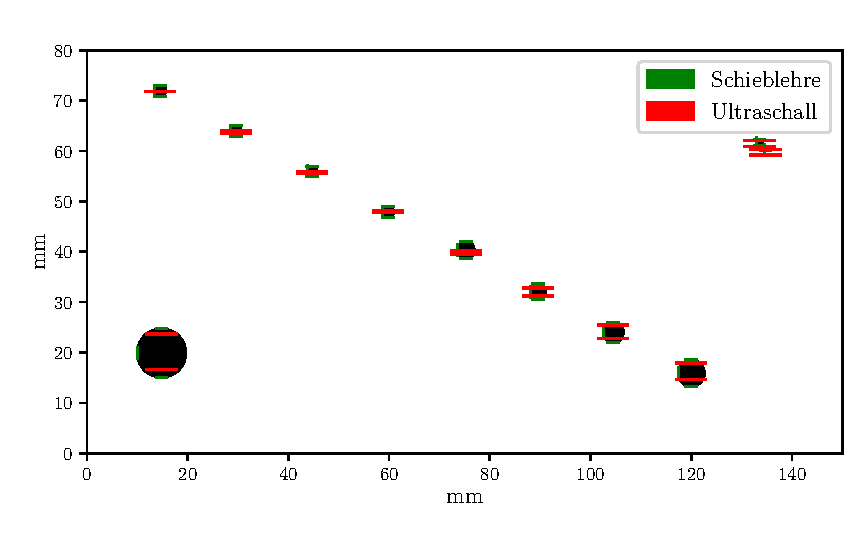
\includegraphics[width=\textwidth]{build/plt/visualization.pdf}
  \caption{Darstellung aller gemessenen Distanzen.}
  \label{fig:plt:visualization}
\end{figure}

\subsection{Bestimmung des Absorptionskoeffizienten von Acryl}
\label{sec:auswertung:absorptionskoeffizient}

Aus \autoref{eqn:absorptionskurve} ist bekannt,
dass die Intensität des Ultraschalls exponentiell mit der Eindringtiefe und einem Parameter $\alpha$ abfällt.
Daher kann mittels Logarithmieren und linearer Regression $\alpha$ schnell zu
\[ \alpha = \SI{17.6(27)}{\per\meter} \]
bestimmt werden.
Hierbei kommen die mit der Schieblehre gemessenen Distanzen
und die mit der Ultraschallsonde gemessenen Echo-Zeiten zum Einsatz.
% TODO: Besseres Wort für „Zeiten“?
Ein Plot von Messwerten und Regressiongerade ist in \autoref{fig:plt:absorptionskurve} zu sehen.

\begin{figure}
  \centering
  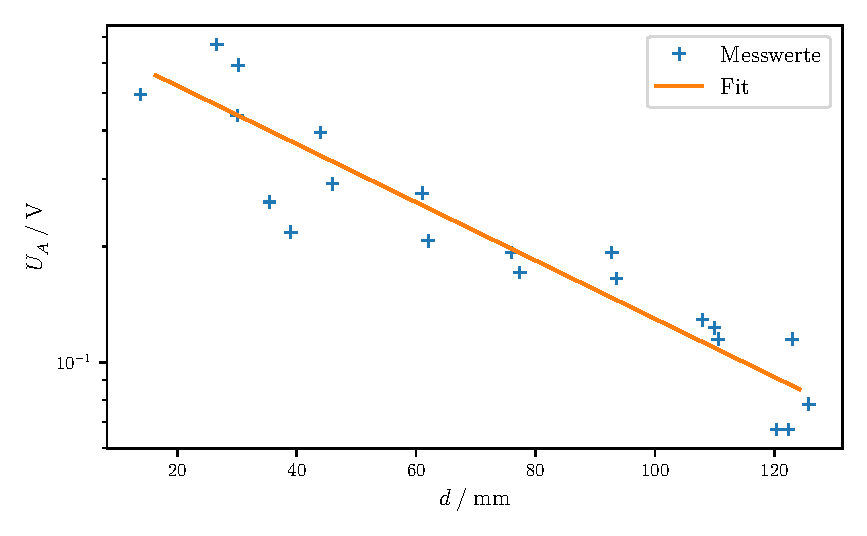
\includegraphics[width=\textwidth]{build/plt/absorptionskurve.pdf}
  \caption{Intensität des Echos ausgedrückt durch die Spannung,
  logarithmisch aufgetragen gegen den Abstand der Fehlstelle.}
  \label{fig:plt:absorptionskurve}
\end{figure}

\FloatBarrier
\subsection{Untersuchung eines Augenmodells}
\label{sec:auswertung:augenmodell}

Mit dem schon zuvor verwendeten Impuls-Echo-Verfahren
%und der Darstellung als A-Scan
wird schließlich ein Augenmodell untersucht.
Es wurden die Echo-Zeiten für die erkennbaren Peaks im Zeit-Spektrum festgehalten.
Aus diesen und den bekannten Schallgeschwindigkeiten
für Linse
\begin{align*}
c_\text{L} &= \SI{2500}{\meter\per\second} \\
\intertext{und Glaskörperflüssigkeit}
c_\text{GK} &= \SI{1410}{\meter\per\second} \\
\end{align*}
sowie den Daten des A-Scans
lassen sich dann die Abmessungen des Augenmodells berechnen.
Die Resultate sind in \autoref{tab:augenmodell} aufgeführt.

\begin{table}
  \centering
  \caption{Echo-Zeiten und berechnete Abmessungen des Augenmodells unter Angabe der jeweils verwendeten Schallgeschwindigkeit.}
  \label{tab:augenmodell}
  \sisetup{table-format=2.1} % TODO: lol?
  \begin{tabular}{c S c S S}
  \toprule
  Strecke &
  {Zeit [$\si{\micro\second}$]} &
  Schallgeschwindigkeit &
  {rel. Distanz [$\si{\milli\meter}$]} &
  {abs. Distanz [$\si{\milli\meter}$]} \\
  \midrule
  Hornhaut – Linse    & 11.7 & $c_\text{GK}$ & 8.249 &  8.249 \\
  Innerhalb der Linse &  4.5 & $c_\text{L}$  & 5.625 & 13.874 \\
  Linse – Retina      &  6.6 & $c_\text{GK}$ & 4.653 & 18.527 \\
  \bottomrule
  \end{tabular}
\end{table}
